\documentclass[12pt]{article}
%% arXiv paper template by Flip Tanedo
%% last updated: Dec 2016


%%%%%%%%%%%%%%%%%%%%%%%%%%%%%
%%%  THE USUAL PACKAGES  %%%%
%%%%%%%%%%%%%%%%%%%%%%%%%%%%%

\usepackage{amsmath}
\usepackage{amssymb}
\usepackage{amsfonts}
\usepackage{graphicx}
\usepackage{xcolor}
\usepackage{nopageno}
\usepackage{enumerate}
\usepackage{parskip}

%%%%%%%%%%%%%%%%%%%%%%%%%%%%%%%%%
%%%  UNUSUAL PACKAGES        %%%%
%%%  Uncomment as necessary. %%%%
%%%%%%%%%%%%%%%%%%%%%%%%%%%%%%%%%

%% MATH AND PHYSICS SYMBOLS
%% ------------------------
%\usepackage{slashed}       % \slashed{k}
%\usepackage{mathrsfs}      % Weinberg-esque letters
%\usepackage{youngtab}	    % Young Tableaux
%\usepackage{pifont}        % check marks
\usepackage{bbm}           % \mathbbm{1} incomp. w/ XeLaTeX 
%\usepackage[normalem]{ulem} % for \sout


%% CONTENT FORMAT AND DESIGN (below for general formatting)
%% --------------------------------------------------------
\usepackage{lipsum}        % block of text (formatting test)
%\usepackage{color}         % \color{...}, colored text
%\usepackage{framed}        % boxed remarks
%\usepackage{subcaption}    % subfigures; subfig depreciated
%\usepackage{paralist}      % compactitem
%\usepackage{appendix}      % subappendices
%\usepackage{cite}          % group cites (conflict: collref)
%\usepackage{tocloft}       % Table of Contents	

%% TABLES IN LaTeX
%% ---------------
%\usepackage{booktabs}      % professional tables
%\usepackage{nicefrac}      % fractions in tables,
%\usepackage{multirow}      % multirow elements in a table
%\usepackage{arydshln} 	    % dashed lines in arrays

%% Other Packages and Notes
%% ------------------------
%\usepackage[font=small]{caption} % caption font is small



\renewcommand{\thesection}{}
\renewcommand{\thesubsection}{\arabic{subsection}}

%%%%%%%%%%%%%%%%%%%%%%%%%%%%%%%%%%%%%%%%%%%%%%%
%%%  PAGE FORMATTING and (RE)NEW COMMANDS  %%%%
%%%%%%%%%%%%%%%%%%%%%%%%%%%%%%%%%%%%%%%%%%%%%%%

\usepackage[margin=2cm]{geometry}   % reasonable margins

\graphicspath{{figures/}}	        % set directory for figures

% for capitalized things
\newcommand{\acro}[1]{\textsc{\MakeLowercase{#1}}}    

\numberwithin{equation}{subsection}    % set equation numbering
\renewcommand{\tilde}{\widetilde}   % tilde over characters
\renewcommand{\vec}[1]{\mathbf{#1}} % vectors are boldface

\newcommand{\dbar}{d\mkern-6mu\mathchar'26}    % for d/2pi
\newcommand{\ket}[1]{\left|#1\right\rangle}    % <#1|
\newcommand{\bra}[1]{\left\langle#1\right|}    % |#1>
\newcommand{\Xmark}{\text{\sffamily X}}        % cross out


\let\olditemize\itemize
\renewcommand{\itemize}{
  \olditemize
  \setlength{\itemsep}{1pt}
  \setlength{\parskip}{0pt}
  \setlength{\parsep}{0pt}
}


% Commands for temporary comments
\newcommand{\comment}[2]{\textcolor{red}{[\textbf{#1} #2]}}
\newcommand{\flip}[1]{{\color{red} [\textbf{Flip}: {#1}]}}
\newcommand{\email}[1]{\texttt{\href{mailto:#1}{#1}}}

\newenvironment{institutions}[1][2em]{\begin{list}{}{\setlength\leftmargin{#1}\setlength\rightmargin{#1}}\item[]}{\end{list}}


\usepackage{fancyhdr}		% to put preprint number



%%%%%%%%%%%%%%%%%%%
%%%  HYPERREF  %%%%
%%%%%%%%%%%%%%%%%%%

%% This package has to be at the end; can lead to conflicts
\usepackage{microtype}
\usepackage[
	colorlinks=true,
	citecolor=black,
	linkcolor=black,
	urlcolor=green!50!black,
	hypertexnames=false]{hyperref}



%%%%%%%%%%%%%%%%%%%%%
%%%  TITLE DATA  %%%%
%%%%%%%%%%%%%%%%%%%%%

\begin{document}


\begin{center}

    {\Large \textsc{Homework 2b:} 
    \textbf{What is a Green's Function}}
    
\end{center}

\vskip .4cm

\noindent
\begin{tabular*}{\textwidth}{rlcrll}
	\textsc{Course:}& Physics 231, \emph{Methods of Theoretical Physics} (2018)
	&
%	\hspace{1.2cm}
	&
	\\
	\textsc{Instructor:}& Professor Flip Tanedo (\email{flip.tanedo@ucr.edu})
	&
	%\hfill
	&
	& 
	\\
	\textsc{Due by:}& Mon, October 29
	&
	%\hfill
	&
	%	
\end{tabular*}







\subsection{A Green's function by completeness}

Three formulaic ways of solving for Green's functions are:
\begin{enumerate}
	\item Fourier transforming to turn the differential operator into an algebraic one, and then doing a contour integral to go back to position space.
	\item Solving the homogeneous equation and patching together two solutions over the $\delta$-function. 
	\item Using the completeness of eigenfunctions.
\end{enumerate}
We will spend most of this course highlighting method 1. Method 2 will be familiar from electrodynamics. Here we use the third method, which is based on the eigenfunction completeness relation,
\begin{align}
	\sum_n e_n^*(y) e_n(x) = \delta(x-y) \ .
\end{align}
If you know the eigenvalues of the linear differential operator, $L_x$, then you can use this relation to hack together the Green's function $G$ because $L_x G(x,y) = \delta(x-y)$.  The subscript $x$ in $L_x$ means that the operator is a function of $x$ and derivative operators with respect to $x$.

\textsc{References}: This method is discussed in  Matthews \& Walker chapter 9-4, Stone \& Goldbart chapter 5.4, Cahill chapter 6.38, and Byron \& Fuller chapter 7.2. 

In this problem, we consider a second order differential equation acting on a state $\psi(x)$ with a source $s(x)$. 
\begin{align*}
	\left(-\frac{d^2}{dx^2} + k^2 \right) \psi(x) = s(x) \ .
\end{align*}
We consider the domain $x\in[0,1]$ with boundary conditions $\psi(0) = \psi(1) = 0$.

\subsubsection{Eigenfunctions}

What are the eigenfunctions $e_n(x)$ and the corresponding eigenvalues $\lambda_n$? Recall that an eigenfunction of a linear operator $L_x$ satisfies $L_x e_n(x) = \lambda_n e_n(x)$. 


\textsc{Hint:} The eigenfunctions of $-d^2/dx^2$ are $\psi_n(x) = \sqrt{2} \sin (n\pi x)$ with eigenvalues $n^2 \pi^2$. What changes when the operator $L_x$ includes an additive constant?


\subsubsection{Completeness}


Write down the Green's function $G(x,y)$ using the completeness trick with respect to eigenfunctions $e_n$ with eigenvalues $\lambda_n$: 
\begin{align}
	G(x,y) = \sum_n \frac{e_n^*(y)e_n(x)}{\lambda_n} \ .
\end{align}

\textsc{Hint:} Once you did the previous part, this step takes about twenty seconds depending on how quickly you write.


\subsubsection{Hands on}

You have a free license for several types of scientific software 
through \acro{UCR} through MySoftware\footnote{\url{http://cnc.ucr.edu/mysoftware/}}. This problem requires some plotting. I suggest using \emph{Mathematica}\footnote{It sucks that this is not open source software. The closest open source alternative is \texttt{SciPy} with a \texttt{Jupyer} notebook.}. 

Plot the solution to the Green's function $G(x,y)$ for $y = 0.5$ and $k = 0.2$, summing from $n=1$ to $n=10$. Here's the general way to format it in \emph{Mathematica}:
\begin{center}
	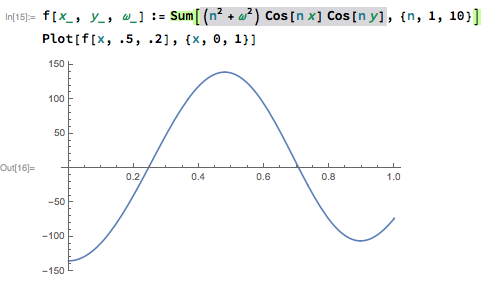
\includegraphics[width=.6\textwidth]{P231_2017_HW4_fig1.png}
\end{center}

The highlighted piece and the example plot are \emph{completely wrong}! Fill it in with the correct $G(x,y)$ and plot it. It may help to use the `Basic Math Input' palette if you're unfamiliar with this. If this task is very painful, please ask a friend. If this is still very painful, then you may use any other plotting program that you wish. 

Does this shape make sense? What do you expect will happen as $n$ becomes larger? Try it for $n=100$. Explore what happens as you change $k$ and $y$. (Make sure $y$ is in the domain of the function space!) Take a moment to have a nice warm cup of tea, enjoy the agreeable weather outside, and meditate upon why this shape of the Green's function makes sense and the kinds of physical problem where Green's function may be relevant. You do not have to write up these meditations, but I do strongly suggest the tea and outdoors.  




\subsection{A Green's function by patching}

\emph{This looks like a long problem, but it's mostly reading and understanding. Each step is modest.}

In this problem we solve for a Green's function by patching together solutions of the homogeneous equation.  We examine the same system that you did in Homework 4, Problem \#2: consider a second order differential equation acting on a state $\psi(x)$ with a source $s(x)$. 
\begin{align*}
\mathcal O \psi(x) = 
	\left(-\frac{d^2}{dx^2} + k^2 \right) \psi(x) = s(x) \ .
\end{align*}
We consider the domain $x\in[0,1]$ with boundary conditions $\psi(0) = \psi(1) = 0$. \textbf{For simplicity}, we'll take $k^2 = 0$ and leave the $k^2 \neq 0$ case for extra credit.



We want to solve the Green's function equation, $$\mathcal O G(x,y) = \delta(x-y)\, .$$ In this method, we solve the \emph{homogeneous} equation $\mathcal O G(x,y) = 0$ for $x\neq y$ in the two regions $x<y$ and $x>y$. These two solutions will each have independent coefficients that we must patch together at $x=y$.

\subsubsection{Solve the homogeneous equation}

Solve the two \emph{homogeneous} equations in the regions away from the $\delta$-function spike:
\begin{align}
 	-\left(\frac{d}{dx}\right)^2 G_{<}(x,y) = 0  
 	& \quad\text{ in }\quad 0 < x < y \leq 1 
 	\\
 	-\left(\frac{d}{dx}\right)^2 G_{>}(x,y) = 0  
 	& \quad\text{ in }\quad 0 < y < x \leq 1
\end{align}
Don't forget to impose the boundary conditions $G(0, y) = G(L,y) = 0$. Understand why it makes sense that $\psi(0) = \psi(1) = 0$ imposes the same condition on the Green's functions. If the Green's function did not satisfy these conditions, then you could construct sources that violate the boundary conditions because $\psi(1) = \int G(1,y) s(y)\, dy \neq 0$.

The Green's function $G(x,y)$ is now piecewise defined
\begin{align}G(x,y) = \left\{ 
\begin{array}{ll}
 	G_<(x,y) & \quad\text{ if } x<y\\
 	G_>(x,y) & \quad\text{ if } x>y
 \end{array}\right. .
 \label{eq:piecewise:def}
 \end{align}
Check to make sure that you have the correct number of undetermined coefficients. 

\textsc{Hint}: if you're not sure what the solution to the homogeneous differential equation is, then you're over thinking it. It's not a trigonometric function. If you're still confused, refer back to your plot the previous problem.

\subsubsection{Patching, Part 1}
For fixed $y$, integrate the Green's function equation over an infinitesimal sliver, $x \in (y-\varepsilon, y + \varepsilon)$, with $\epsilon \to 0$: 
\begin{align}
	\int_{y-\varepsilon}^{y+\varepsilon} dx\, \left(\frac{d}{dx}\right)^2 G(x,y) &=  
	\int_{y-\varepsilon}^{y+\varepsilon} dx\; \delta(x-y)
	\ .
	\label{eq:patching:1}
\end{align}
\textsc{Hint}: It may be useful to remember that
\begin{align}
	\int_{y-\varepsilon}^{y+\varepsilon} dx\; \frac{df(x)}{dx} = f(y+\epsilon) - f(y-\epsilon) \ .
\end{align}

Write out the resulting equation in terms of $dG_</dx$ and $dG_>/dx$ at $x=y$. You will find that the slope of the Green's function, $dG/dx$, is \emph{discontinuous} at $x=y$. 


\subsubsection{Patching, Part 2}

Integrate (\ref{eq:patching:1}) again over $x\in(y-\epsilon y+\epsilon)$ to relate $G_<$ and $G_>$ at $x=y$.


\textsc{Answer}: $dG/dx$ has a finite discontinuity at $x=y$, therefore $G$ is \emph{continuous} at $x=y$. The discontinuity in the slope gives a kink in $G$,
\begin{align}
	\left.G_<(x, y)\right|_{x=y} &= \left.G_>(x, y)\right|_{x=y} \ .
\end{align}
We've found that the second derivative is a $\delta$-function (singular), the first derivative is simply discontinuous, and the zeroth derivative (the Green's function itself) is continuous.

\subsubsection{Patching, Part 3}

Take all of the above results and write down the piece-wise definition of $G(x,y)$ in (\ref{eq:piecewise:def}) as an explicit function of $x$ and $y$ with all coefficients determined. Sketch $G(x,y)$  for $y=0.5$ and compare it to your plot from Problem \#2.

\subsubsection{Extra Credit: $k^2\neq 0$}

\emph{This problem is not graded and is purely for your ``enjoyment.''} Perform the same steps for the case of $k^2\neq 0$. The homogeneous solution is now a sine, which makes things a bit more complicated. The procedure is completely the same and the $k^2 \lesssim 1$ case is well approximated by $k^2=0$, as you will have noticed from the plot in the previous problem. \textsc{Solution}: Matthews \& Walker, Chapter 9--4. 


\subsection{That funny $i$ in the derivative}

In quantum mechanics, observables are Hermitian (self adjoint) operators. This is important because the value of the observable is a real number and the eigenvalues of Hermitian operators are real. Given that the inner product on our wavefunction space is
\begin{align}
	\langle f | g \rangle = \int dx \; f^*(x) g(x) \ ,
\end{align}
	explain the factor of $i$ in the \textbf{momentum operator}, $\hat p = i\hbar(d/dx)$. Why is this factor of $i$ critical for $\hat p$ to be self adjoint? Show that the eigenvalue of a (momentum eigenstate) plane wave is real. 








\subsection{Practice with complex integration}

\subsubsection{This is not a closed loop}

The goal of this problem is to review line integrals in a 2D space. Perform the integral
\begin{align}
	\int_i^{1+i} dz \; z \,
\end{align}
with respect to the path that connects $z=i$ and $z=i+1$ by a straight line segment. This is \emph{not} a closed loop, there's no magic formula for this. Just parameterize the path by writing $z$ as a function of a real parameter. Then write out $dz$ in terms of the parameter. Do the integral.

\subsubsection{Contour integrals}

Calculate the following integrals using the residue theorem:
\begin{enumerate}[(a)]
	\item $\displaystyle \int_{0}^\infty \frac{x^2}{x^4 + 16} dx$ 
	\item $\displaystyle \int_{-\infty}^\infty \frac{\sin x}{x^2 + 4x + 5}dx$ 
	\item $\displaystyle \int_{0}^\infty \frac{1}{x^6+1}dx$ using a contour including the real line and a large semicircle in the complex plane 
	\item $\displaystyle \int_{0}^\infty \frac{1}{x^6+1}dx$ using a contour that encloses the `pizza slice' wedge between $\theta = 0$ and $\theta = \pi/3$. 
\end{enumerate}

\textsc{Hint}: for (d), the line integral along the diagonal is proportional to the integral you want. 




\subsection{How to find Residues}

This problem is based on Boas (page 599) and Appel (section 4.5d).
%
We saw that a \textbf{meromorphic} (analytic up to poles) function has a Laurent series expansion about a point $z_0$,
\begin{align}
f(z) &= \sum_{n=-\infty}^{\infty} a_n (z-z_0)^n
	\ .
\end{align}
The $a_{-1}$ term has special significance and is known as the \textbf{residue} of $f$ at $z_0$, $\text{Res}(f,z_0)$. When we have an explicit Laurent expansion about $z_0$, identifying the residue is a matter of reading off the $(z-z_0)^{-1}$ coefficient. Alternately, when $z_0$ is a simple pole the function can be written as
\begin{align}
	f(z) = \frac{F(z)}{(z-z_0)} \ ,
\end{align}
where $F(z)$ is analytic at $z_0$. In this case, the residue is $\text{Res}(f,z_0) = F(z_0)$. This leads to the sometimes useful guide: If $f(z_0)$ is not finite but $(z-z_0)\, f(z)$ is finite, then
	\begin{align}
		\text{Res}(f,z_0) &=  \lim_{z\to z_0} (z-z_0)\, f(z) \ .
	\end{align}
What do we do if $(z-z_0)\, f(z)$ is \emph{not} finite? For example, what if both $a_{-1}$ and $a_{-2}$ were non-zero? How does determine the residue ($a_1$) in such a case? Explain why the following algorithm works: Find the positive integer $m$ such that $F_m(z)=(z-z_0)^m f(z)$ is finite at $z=z_0$, then the residue is
\begin{align}
	\text{Res}(f,z_0) = \left.\frac{1}{(m-1)!} \frac{d^{m-1}}{dz^{m-1}} F_m(z)\right|_{z=z_0} \ .
\end{align}











\section{Extra Credit}

These problems are not graded and are for your edification. You are strongly encouraged to explore and discuss these topics, especially if they are in a field of interest to you.



\subsection{A two-dimensional function space} 


Let us ignore the subtleties of defining a function space (metric, domain, boundary conditions). Instead, let's construct a cute two-dimensional function space that gives us a shortcut to calculate a particular \emph{indefinite} integral. 

Consider a two dimensional vector space spanned by the functions
\begin{align}
	\left|f_1\right\rangle
	&= f_1(x) = 
	e^{ax} \cos bx
	&
	\left|f_2\right\rangle
	&=
	f_2(x) = 
	e^{ax} \sin bx \ ,
\end{align}
where $a$ and $b$ are constants. Forget orthonormality or boundary conditions for this problem. The derivative $d/dx$ is a linear operator that acts on this space. Write down the derivative as a $2\times 2$ matrix in the above basis, $D$.

Invert $D$ in the usual way that you learned to invert $2\times 2$ matrices during your childhood\footnote{Stuck? Here's a life pro tip: \url{http://bfy.tw/KG2Z}}. Call this matrix $D^{-1}$. 

Now stop and think: the inverse of a derivative is an indefinite integral\footnote{Ignore the constant term.}. Thus acting with $D^{-1}$ on the vector $|f_1\rangle$ should be understood as an integral of $f_1(x)$. Show that, indeed,
\begin{align}
	D^{-1} |f_1\rangle = \int dx\, e^{ax} \cos bx \ .
\end{align}
Feel free to use \emph{Mathematica} to do the indefinite integral on the right-hand side. Pat yourself on the back if you can do it without a computer.







\subsection{Black Hole Entropy and Dimensional Analysis}

This problem is from Tony Zee's \emph{Einstein Gravity in a Nutshell}. This is recommended for those interested in cosmology and condensed matter physics.

\subsubsection{The Planck Mass}

In natural units, the Newton constant $G$ has [mass] dimension $[G] = -2$ (here we're using natural units---see HW1b, extra credit problem 2), so that we can define a mass scale
\begin{align}
	M_P = \frac{1}{\sqrt{G}} \ .
\end{align}
This is called the \textbf{Planck mass}. Restore the factors of $\hbar$ and $c$ to make this definition correct in `unnatural' units where we keep track of length and time dimensions.

\subsubsection{Hawking Radiation}

Black holes can evaporate by Hawking radiation. A cartoon picture of this process is as follows: quantum mechanics + special relativity tells us that the vacuum (`empty' space) is composed of virtual particle--anti-particle pairs. Near the event horizon of a black hole, one of these particles can fall into the black hole while the other radiates away as a physical particle. This means that black holes have a temperature. 

Use dimensional analysis to determine how this \textbf{Hawking temperature} scales with the mass of the black hole. How does $T_H$ scale with the combination $GM$? Observe that the black hole gets \emph{hotter} as it loses energy.


\textsc{Hint}: there's one subtlety. There are two mass scales in the problem: the black hole mass, $M$, and the Planck mass, $M_P = 1/\sqrt{G}$. (In natural units, of course). In order to be able to use dimensional analysis, the additional piece of information is that $G$ is a gravitational coupling, so that gravitational effects should go like $GM$. 


\subsubsection{The Holographic Principle}

Recall from thermodynamics that entropy, $S$, is related to energy $E$ and temperature $T$ by
\begin{align}
	\frac{dS}{dE} = \frac{1}{T} \ .
\end{align}
\begin{enumerate}[(i)]
	\item Identify the temperature with the Hawking temperature $T=T_H$ and set the energy to be the mass of the black hole so that $dE = dM$. Integrate with respect to the black hole mass to find how entropy scales with mass, $S \sim M^?$.
	\item The radius of the black hole's event horizon scales like $R = GM$. How does the black hole's entropy scale with its characteristic length scale? 
	\item Contrast the above result to the expected scaling of entropy in ordinary thermodynamics. Recall that entropy is an \emph{extensive}\footnote{An \textbf{extensive} property is one that adds for separate subsystem. Consider a system of two lazy cats. The mass of the combined system is equal to the sum of the masses of each cat. This is in contrast to temperature, which is \textbf{intensive}; the temperature of the multi-lazy-cat system is $T_\text{cat}$ to matter how many cats there are. This example obviously breaks down at large numbers of cats.} measure of the number of microstates in a system.
\end{enumerate}

The solution to this problem is spelled out in  the introduction to Zee's \emph{Einstein's Gravity in a Nutshell}. The `holographic principle' is the proposal that the properties of the black hole are encoded on its surface rather than its volume. This is analogous to how a hologram is a 3D image encoded onto a 2D surface. A manifestation of the holographic principle is the AdS/CFT correspondence, which posits that certain theories of strongly interacting systems in $d$-dimensions are mathematically identical to a weakly-coupled $(d+1)$-dimensional gravitational theory.




\subsection{Renormalization Group as Dimensional Analysis}

This problem is recommended for particle/nuclear physicists and especially to theorists of any type.

Read the paper ``Dimensional Analysis in Field Theory: An Elementary Introduction to Broken Scale Invariance and the Renormalization Group Equations'' by Paul Stevenson\footnote{Annals Phys. \textbf{132} (1981) 383, \url{http://dx.doi.org/10.1016/0003-4916(81)90072-5}}. This paper describes the phenomenon of dimensional transmutation in quantum/statistical field theory in a way that strips it of the mysticism that tends to appear when you first learn field theory. In particular, it explains why dimensionless `coupling constants' are not really constant and are scale dependent. Understand the  dimensional analysis theorem in the paper and then understand how that theorem is evaded in actual physics. Theorists should take time to understand this paper carefully.\


\subsection{Sturm--Liouville Operator}

This question is based on Matthews \& Walker, chapter 9--2 and/or Stone \& Goldbart chapter 4.2. Consider the \textbf{Sturm--Liouville} differential operator
\begin{align}
	L = p_2(x) \left(\frac{d}{dx}\right)^2
	+ p_1(x)\frac{d}{dx}
	+ p_0(x) .
\end{align}
Assume weight $w(x) = 1$ and some domain $x\in [a,b]$.

%\textsc{Reference}: Refer to Stone \& Goldbart chapter 4 for a discussion of formal versus concrete (what we called `proper') linear differential operators. We use a slightly different notation, but the question of a formal adjoint is explored in 4.2 with the Sturm--Liouville operator identified in equation (4.28). A more general discussion that follows more of the spirit of the lecture is in Matthews \& Walker Chapter 9-2.

\subsubsection{Formal adjoint}
Using integration by parts, show that the \textbf{formal adjoint} of this operator is 
\begin{align}
	L^\dag = \left(\frac{d}{dx}\right)^2 p_2(x)
	- \left(\frac{d}{dx}\right)p_1(x)
	+ p_0(x) \ ,
\end{align}
where we use the notation 
\begin{align}
	\left[\left(\frac{d}{dx}\right)^n p_n(x)\right] f(x) \equiv 
		\left(\frac{d}{dx}\right)^n 
		\left[ p_n(x)\, f(x)\right] \ .
\end{align}

\subsubsection{Self-Adjoint Case}

Show that in order for $L$ to be formally self-adjoint, that is $L = L^\dag$ (without considering boundary conditions), then the following conditions must hold:
\begin{align}
	p_1(x) &= 2p_2'(x) - p_1(x) \\
	p_0(x) &= p_x''(x) - p_1(x) + p_0(x) \ .
\end{align}
Thus $L$ is self-adjoint (Hermitian) if $p_1(x) = p_2'(x)$. $L$ can be written succinctly as:
\begin{align}
	L &= \frac{d}{dx}
		\left(p_2(x)\frac{d}{dx}\right) + p_0(x) \ .
\end{align}




\end{document}